
\subsection{CLU}
\label{sec:algorithms:clu}

CLU, short for Co-Optimizing Locality and Utility, is an algorithm presented by D. Zhan et al.~\cite{Zhan2014} in 2014.
The authors of CLU recognize that recent research in LLC partitioning has followed two distinct directions.
Some publications optimize for access locality and attempts to improve performance by changing the lifetime of blocks in LRU managed caches.
DIP, TADIP, and NUCache are three such solutions that use novel methods to reduce or extend the lifetime of blocks in an elsewise LRU managed cache.
Other publications recognize the usefulness of utility and do way-partitioning between cores based on their utility values.
Examples here are UCP and PIPP.
Because the stack property of LRU is the base of the utility calculations in both PIPP and UCP~\cite{Qureshi2006, Xie2009}, they cannot evaluate the utility of algorithms such as DIP's BIP.

The authors of CLU presents a novel approach for calculating the utility curve of a BIP managed cache.
BIP, as covered earlier, is one of the two insertion policies under DIP and TADIP. 
BIP violates the stack property of LRU by mostly inserting new rows at the MRU position, or at a low probability in LRU position.
In order to correctly measure the utility curve of a BIP managed k-way cache, one needs k ATDs; ATD($1$), ATD($2$), ... ATD($k$). 
Where ATD($x$) is an x-way ATD.
In contrast, the utility curve of an LRU managed cache can be found using one ATD, due to the stack property.
Having k ATDs per core sharing the LLC is not a realistic goal due to the required overhead.
The authors of CLU proposes a simplification where there are $m = log_2 k$ ATDs; ATD($1$), ATD($2^1$), ..., ATD($2^m$).
A linear increase between the sample points is assumed when calculating the final utility curve.
It should be noted that the storage overhead of m ATDs in total is less the twice the overhead of the single ATD($k$) required to sample the LRU curve.

CLU uses the two curves first to allocate ways to each core using the same algorithm as shown for UCP in section~\ref{sec:algorithms:ucp}.
The only difference is that the algorithm uses either the LRU of BIP value when estimating utility given an allocation, depending on which algorithm performs best.
During runtime, CLU works like UCP.
The only exception is that the cores ways are managed by either LRU or BIP, depending on which algorithm has the best utility value for the number of ways currently assigned to that core.

\begin{figure}[ht]
    \centering
    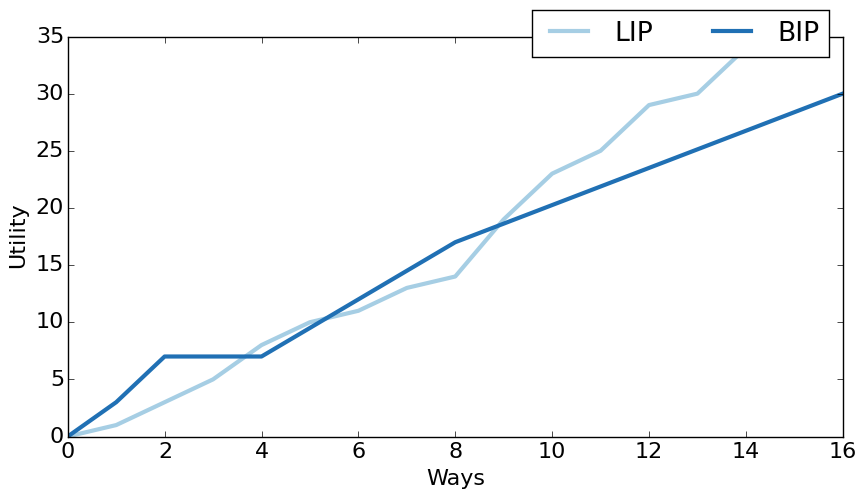
\includegraphics[width=.65\textwidth]{figures/algorithms/clu-utility}
    \caption{Utility plot of BIP and LIP for a 16-way cache.}
    \label{fig:algorithms:lru_example}
\end{figure}

\todo{Create a sample plot with a dummy lru and bip utility line as an illustration}